\documentclass{beamer}
%\documentclass[xcolor=dvipsnames]{beamer}
\usepackage[spanish]{babel}
\usepackage[utf8]{inputenc}
\usepackage{graphicx}
\usepackage{latexsym}

\newcommand{\beamer}{\textsc{beamer}}
\newtheorem{definicion}{Definición}
\newtheorem{ejemplo}{Ejemplo}

%%%%%%%%%%%%%%%%%%%%%%%%%%%%%%%%%%%%%%%%%%%%%%%%%%%%%%%%%%%%%%%%%%%%%%%%%%%%%%%
\title[Hadoop - MapReduce]{Hadoop - MapReduce \\
Restaurants close to Tenerife's beaches}

\author[Juan José Labrador González] {
Juan José Labrador González \\
}

\institute[ULL]{Escuela Superior de Ingeniería y Tecnología \\
                Computación de Altas Prestaciones y Tecnologías Web \\
                Máster en Ingeniería Informática \\
                Universidad de La Laguna}
\date[01-06-2015]{01 de Junio de 2015}
%%%%%%%%%%%%%%%%%%%%%%%%%%%%%%%%%%%%%%%%%%%%%%%%%%%%%%%%%%%%%%%%%%%%%%%%%%%%%%%

%\usetheme{Berlin}
\usetheme{Madrid}

%%%%%%%%%%%%%%%%%%%%%%%%%%%%%%%%%%%%%%%%%%%%%%%%%%%%%%%%%%%%%%%%%%%%%%%%%%%%%%%
\definecolor{pantone254}{RGB}{122,59,122}
\definecolor{pantone3015}{RGB}{0,88,147}
\definecolor{pantone432}{RGB}{56,61,66}
\setbeamercolor*{palette primary}{use=structure,fg=white,bg=pantone254}
\setbeamercolor*{palette secondary}{use=structure,fg=white,bg=pantone3015}
\setbeamercolor*{palette tertiary}{use=structure,fg=white,bg=pantone432}
\setbeamercolor*{palette sidebar primary}{use=structure,fg=pantone254}
\setbeamercolor*{palette sidebar tertiary}{use=structure,fg=pantone3015}
\setbeamercolor*{block title}{bg=pantone3015,fg=white}
\setbeamercolor*{alerted text}{fg=pantone432}
\setbeamercolor*{item projected}{fg=pantone254}
\setbeamercolor*{section in toc shaded}{use=structure,fg=structure.fg}
\setbeamercolor*{section in toc}{fg=pantone3015}
\setbeamercolor*{subsection in toc shaded}{fg=pantone3015}
\setbeamercolor*{subsection in toc}{fg=pantone432}

%%%%%%%%%%%%%%%%%%%%%%%%%%%%%%%%%%%%%%%%%%%%%%%%%%%%%%%%%%%%%%%%%%%%%%%%%%%%%%%
\begin{document}
  
%++++++++++++++++++++++++++++++++++++++++++++++++++++++++++++++++++++++++++++++  
\begin{frame}

  \includegraphics[width=0.15\textwidth]{img/ullesc.eps}
  \hspace*{7.5cm}
  \includegraphics[width=0.16\textwidth]{img/etsii.eps}
  \titlepage

\end{frame}
%++++++++++++++++++++++++++++++++++++++++++++++++++++++++++++++++++++++++++++++  

%++++++++++++++++++++++++++++++++++++++++++++++++++++++++++++++++++++++++++++++  
% \begin{frame}
%   \frametitle{Index}  
%   \tableofcontents
% \end{frame}
%++++++++++++++++++++++++++++++++++++++++++++++++++++++++++++++++++++++++++++++  

\section{Goal}
\begin{frame}
  \frametitle{Goal}  
  
  We want to know the closest restaurants of each beach of Tenerife in order to:
  \begin{itemize}
    \item Inform and recommend to the tourist that visit the island where they can take a meal.
    \item Give new gastronomic options to the Tenerife population.
    \item Promote new restaurants.
  \end{itemize}
  
\end{frame}
%++++++++++++++++++++++++++++++++++++++++++++++++++++++++++++++++++++++++++++++  

\section{Solution}
\begin{frame}
  \frametitle{Solution}
  
  \begin{itemize}
    \item We use {\bfseries Hadoop-MapReduce} to solve this approach.
    \item The input files of beaches and restaurants come from {\bfseries OpenData Canarias}, 
    specifically from {\bfseries SPET, Turismo de Tenerife S.A.} Dataset.
    \newline
    \begin{center}
      
\includegraphics[width=0.3\textwidth]{img/logo_open-02.eps}
      \newline
      %\hspace*{0.8cm}
      %
\includegraphics[width=0.2\textwidth]{img/turismo-de-tenerife.eps}
    \end{center}
    \item It's possible to change the distance value (in km) for the search.
  \end{itemize}

\end{frame}
%++++++++++++++++++++++++++++++++++++++++++++++++++++++++++++++++++++++++++++++  

\section{Mapper}
\begin{frame}
  \frametitle{Mapper}  
  
  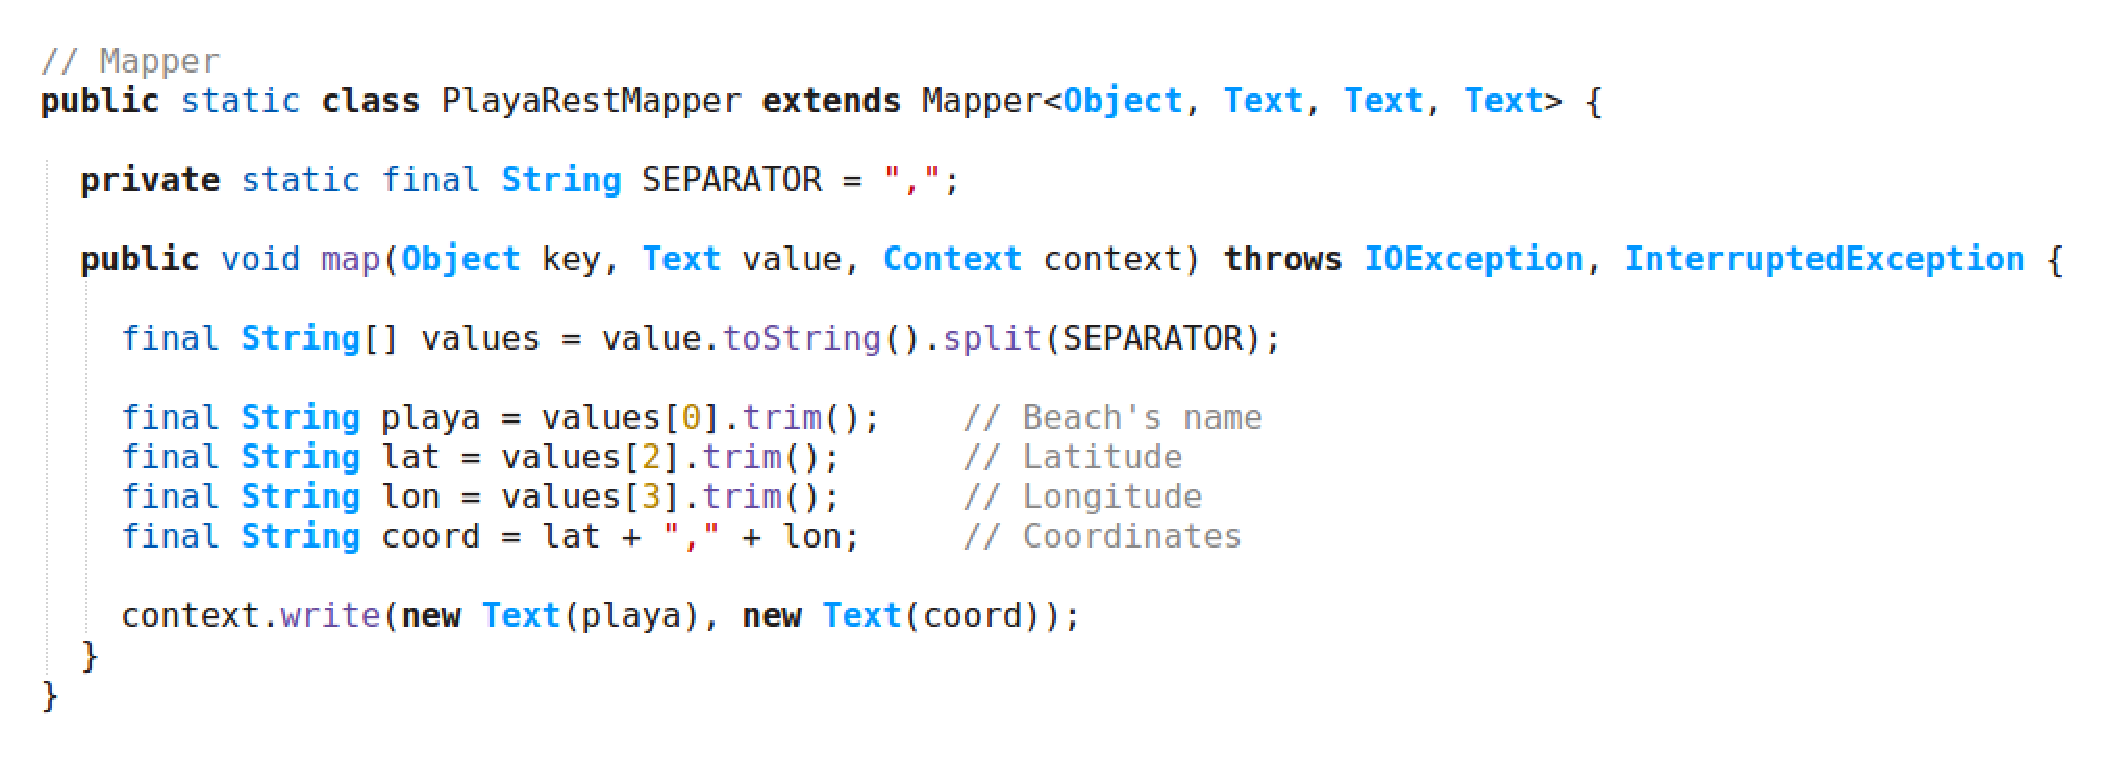
\includegraphics[width=\textwidth]{img/1.eps}
  
\end{frame}
%++++++++++++++++++++++++++++++++++++++++++++++++++++++++++++++++++++++++++++++  

\section{Combiner}
\begin{frame}[allowframebreaks]
  \frametitle{Combiner}  
  
  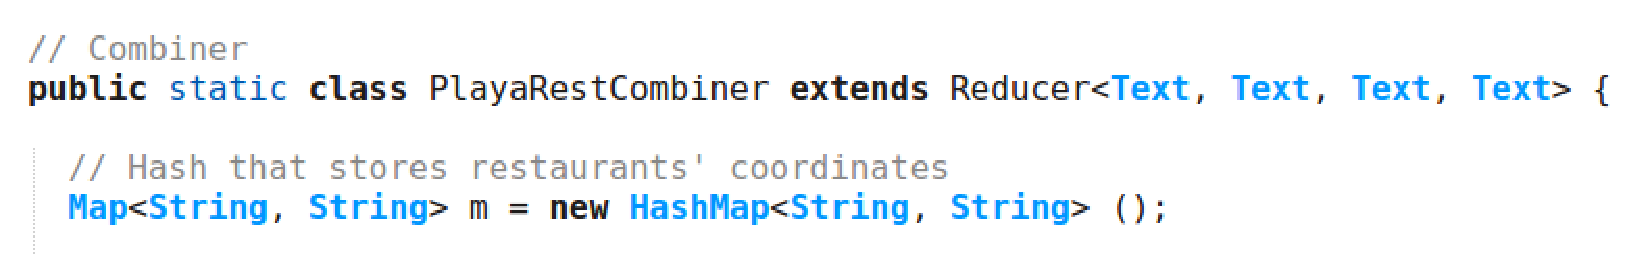
\includegraphics[width=0.9\textwidth]{img/2.eps}
  \hspace*{0.3cm}
  \newline
  \newline
  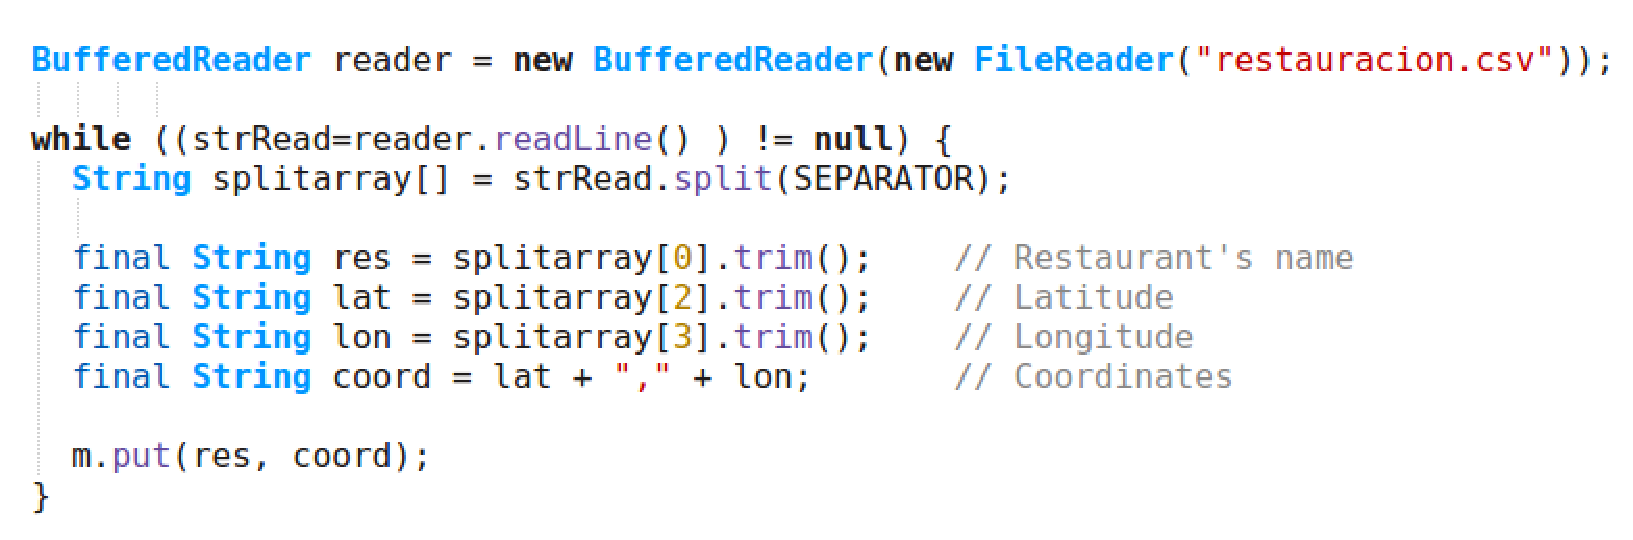
\includegraphics[width=0.9\textwidth]{img/3.eps}
  \framebreak
  %++++++++++++++++++++++++++++++++++++++++++++++++++++++++++++++++++++++++++++++  
  
  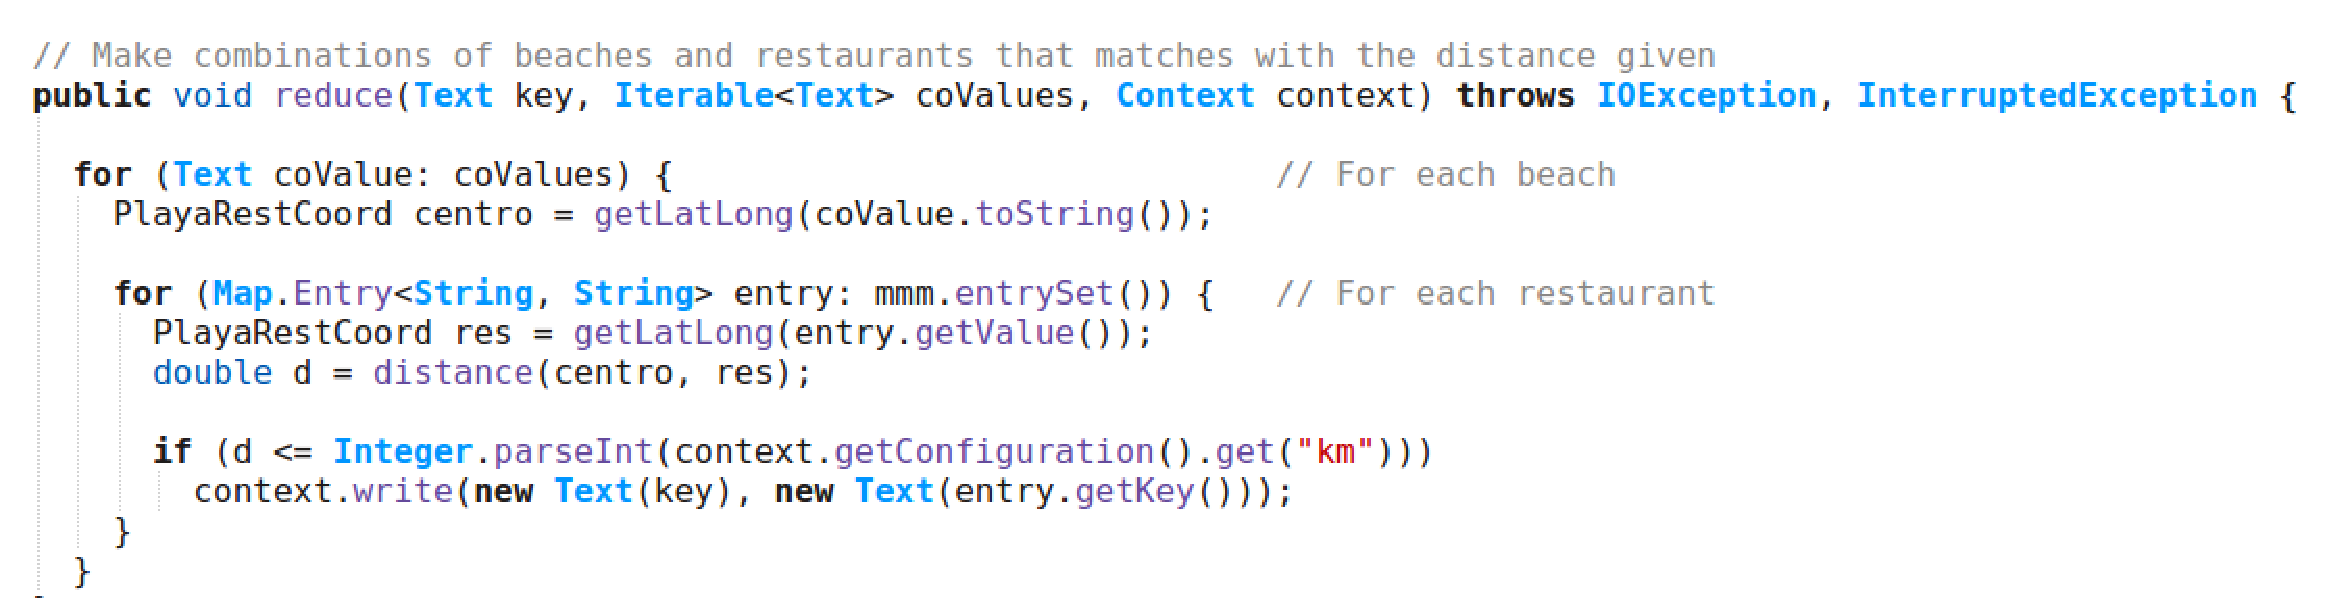
\includegraphics[width=1.05\textwidth,height=4cm]{img/4.eps}
  
\end{frame}
%++++++++++++++++++++++++++++++++++++++++++++++++++++++++++++++++++++++++++++++  

\section{Reducer}
\begin{frame}
  \frametitle{Reducer}  
  
  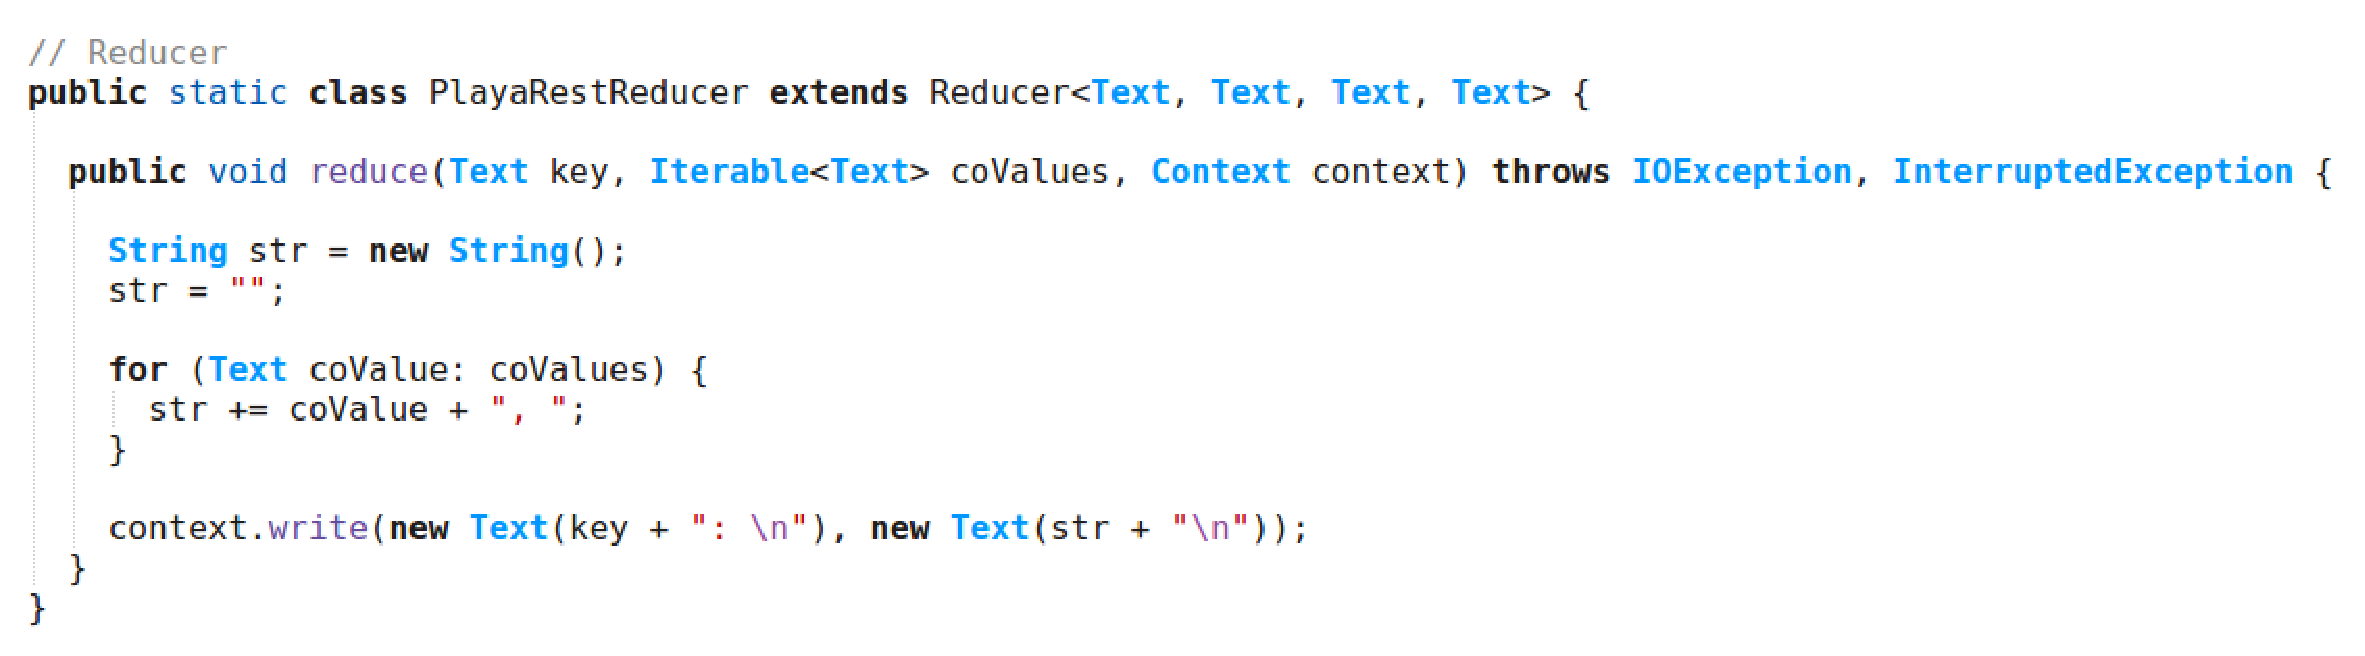
\includegraphics[width=\textwidth,height=4cm]{img/5.eps}

\end{frame}
%++++++++++++++++++++++++++++++++++++++++++++++++++++++++++++++++++++++++++++++  

\section{Running the example}
\begin{frame}
  \frametitle{Running the example}  
  
  {\bfseries bin/hadoop} jar \textless .jar\textgreater \enspace \textless ClassName\textgreater \enspace \textless input dir\textgreater 
  \enspace \textless output dir\textgreater \enspace {\bfseries -files} \textless file.csv\textgreater \enspace {\bfseries -D} \textless distance\textgreater 
  \newline
  
  {\bfseries bin/hadoop} jar pr.jar PlayaRest /user/hduser/input /user/hduser/output {\bfseries -files} /opt/hadoop/jj/restauracion.csv {\bfseries -D} 5
  
\end{frame}
%++++++++++++++++++++++++++++++++++++++++++++++++++++++++++++++++++++++++++++++  

\section{Problems}
\begin{frame}
  \frametitle{Problems}
  \begin{itemize}
    \item Scope of classes' attributes (e.g: between Mappers).
    \item Need of customization of the context for each problem.
    \item Constraint of key-value data.
  \end{itemize}
\end{frame}
%++++++++++++++++++++++++++++++++++++++++++++++++++++++++++++++++++++++++++++++  

\section{Bibliography}
\begin{frame}
  \frametitle{Bibliography}
  \bibliographystyle{ieeetr}
  \bibliography{hadoop}
  \nocite{*}
\end{frame}
%++++++++++++++++++++++++++++++++++++++++++++++++++++++++++++++++++++++++++++++  

\begin{frame}
  \frametitle{End}
  \begin{center}
    \Huge{Thank you}
  \end{center}
\end{frame}

\end{document}